\chapter{Experiments and results}
\label{chap:results}

All results are on held-out \emph{synthetic} data: window-level accuracy on the
test split (\cref{sec:res-window}), event-level detection on a continuous segment
(\cref{sec:event-eval}), robustness to distribution shift (\cref{sec:res-robust})
and computational cost (\cref{sec:res-cost}). \Cref{sec:res-disc} discusses the
trade-offs.

\section{Training dynamics and window-level accuracy}
\label{sec:res-window}

The three models converge within $35$ epochs (\cref{fig:training}). The two
deeper models reach a clearly lower validation loss than the baseline
($\approx 0.57$ for the ResNet and the CNN+Attention vs $\approx 0.72$ for the
1D-CNN) and start higher on validation $F_1$.

\begin{figure}[H]
    \centering
    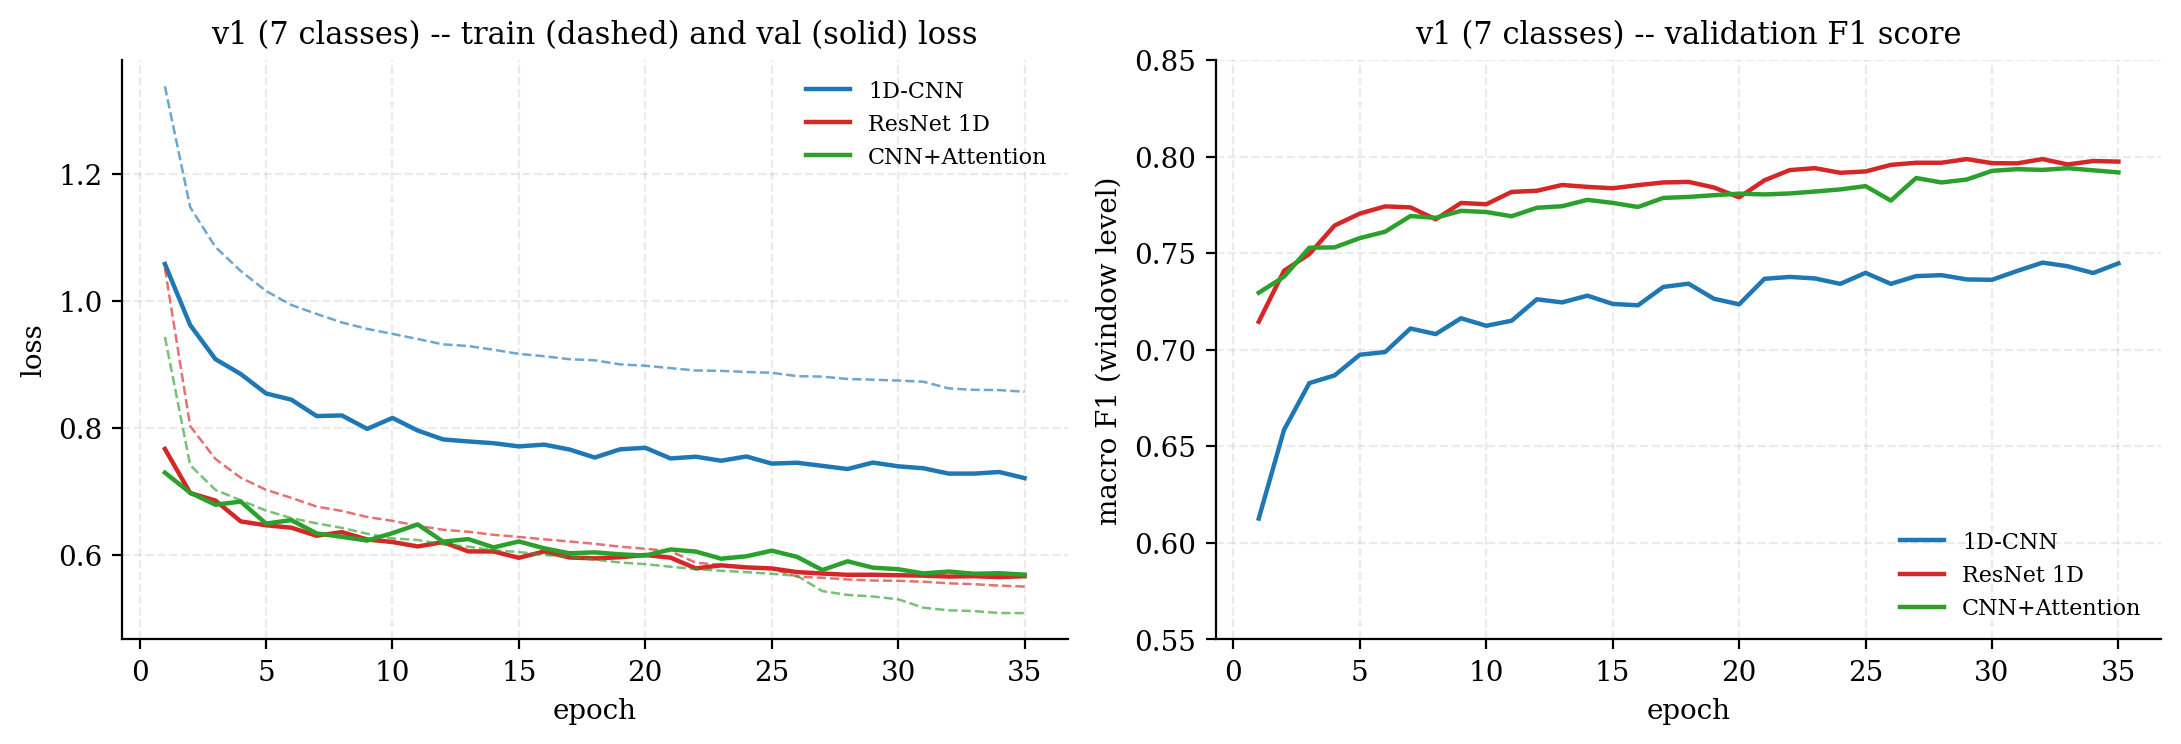
\includegraphics[width=\linewidth]{figures/v1_training_curves}
    \caption{Training dynamics. Train/validation loss (left) and validation macro
    $F_1$ (right) for the three models.}
    \label{fig:training}
\end{figure}

On the $62{,}485$ held-out test windows, the per-class and overall accuracies are
reported in \cref{tab:window-acc}. The background class is recognised at
$\sim 94\%$ by all models; the anomaly classes are harder and tightly grouped,
with \texttt{bell\_sq} the hardest (it is a \texttt{bell} with an added plateau,
easily confused with both \texttt{bell} and \texttt{square}). Depth helps: the
ResNet leads overall, the CNN+Attention is close behind, and both clearly beat
the baseline.

\begin{table}[H]
    \centering \footnotesize
    \begin{tabular}{lccc}
        \toprule
        Class & \textbf{1D-CNN} & \textbf{ResNet 1D} & \textbf{CNN+Attention} \\
        \midrule
        \texttt{Normal Background} & 0.941 & 0.942 & 0.911 \\
        \texttt{bell}              & 0.697 & 0.779 & 0.765 \\
        \texttt{bell\_sq}          & 0.619 & 0.713 & 0.712 \\
        \texttt{fast\_ascend}      & 0.704 & 0.737 & 0.744 \\
        \texttt{fast\_descend}     & 0.721 & 0.741 & 0.738 \\
        \texttt{M}                 & 0.687 & 0.765 & 0.766 \\
        \texttt{square}            & 0.703 & 0.740 & 0.732 \\
        \midrule
        \textbf{Overall accuracy}  & \textbf{0.766} & \textbf{0.807} & \textbf{0.795} \\
        \bottomrule
    \end{tabular}
    \caption{Window-level accuracy on the held-out test set ($62{,}485$ windows).}
    \label{tab:window-acc}
\end{table}

\section{Event-level evaluation}
\label{sec:event-eval}

Window accuracy understates operational quality: the many background windows
inflate it, and boundary windows flip easily. We therefore evaluate detection on
a continuous $100{,}000$-sample segment (immediately after the training portion,
$59$ ground-truth events). The window outputs are averaged into a per-sample
probability trace; a sample is anomalous when its background probability is
below $0.3$; contiguous anomalous runs (gaps up to $50$ samples bridged) form
predicted events, each named by the arg-max of its cumulative probability. A
predicted event matches a true event when their intervals overlap, splitting
results into hits, misses and false alarms, from which we compute precision,
recall and a macro-averaged $F_1$ over the anomaly classes.

\Cref{fig:confmat} shows the event-level confusion matrices and
\cref{tab:event-f1} the summary. The picture is sharp: no model raises a single
false alarm on the segment, and the ranking from \cref{tab:window-acc} is
amplified. The \textbf{ResNet classifies all $59$ events correctly} (macro $F_1
= 1.00$); the CNN+Attention misses $3$ and the 1D-CNN misses $4$, both still
above $0.93$.

\begin{figure}[H]
    \centering
    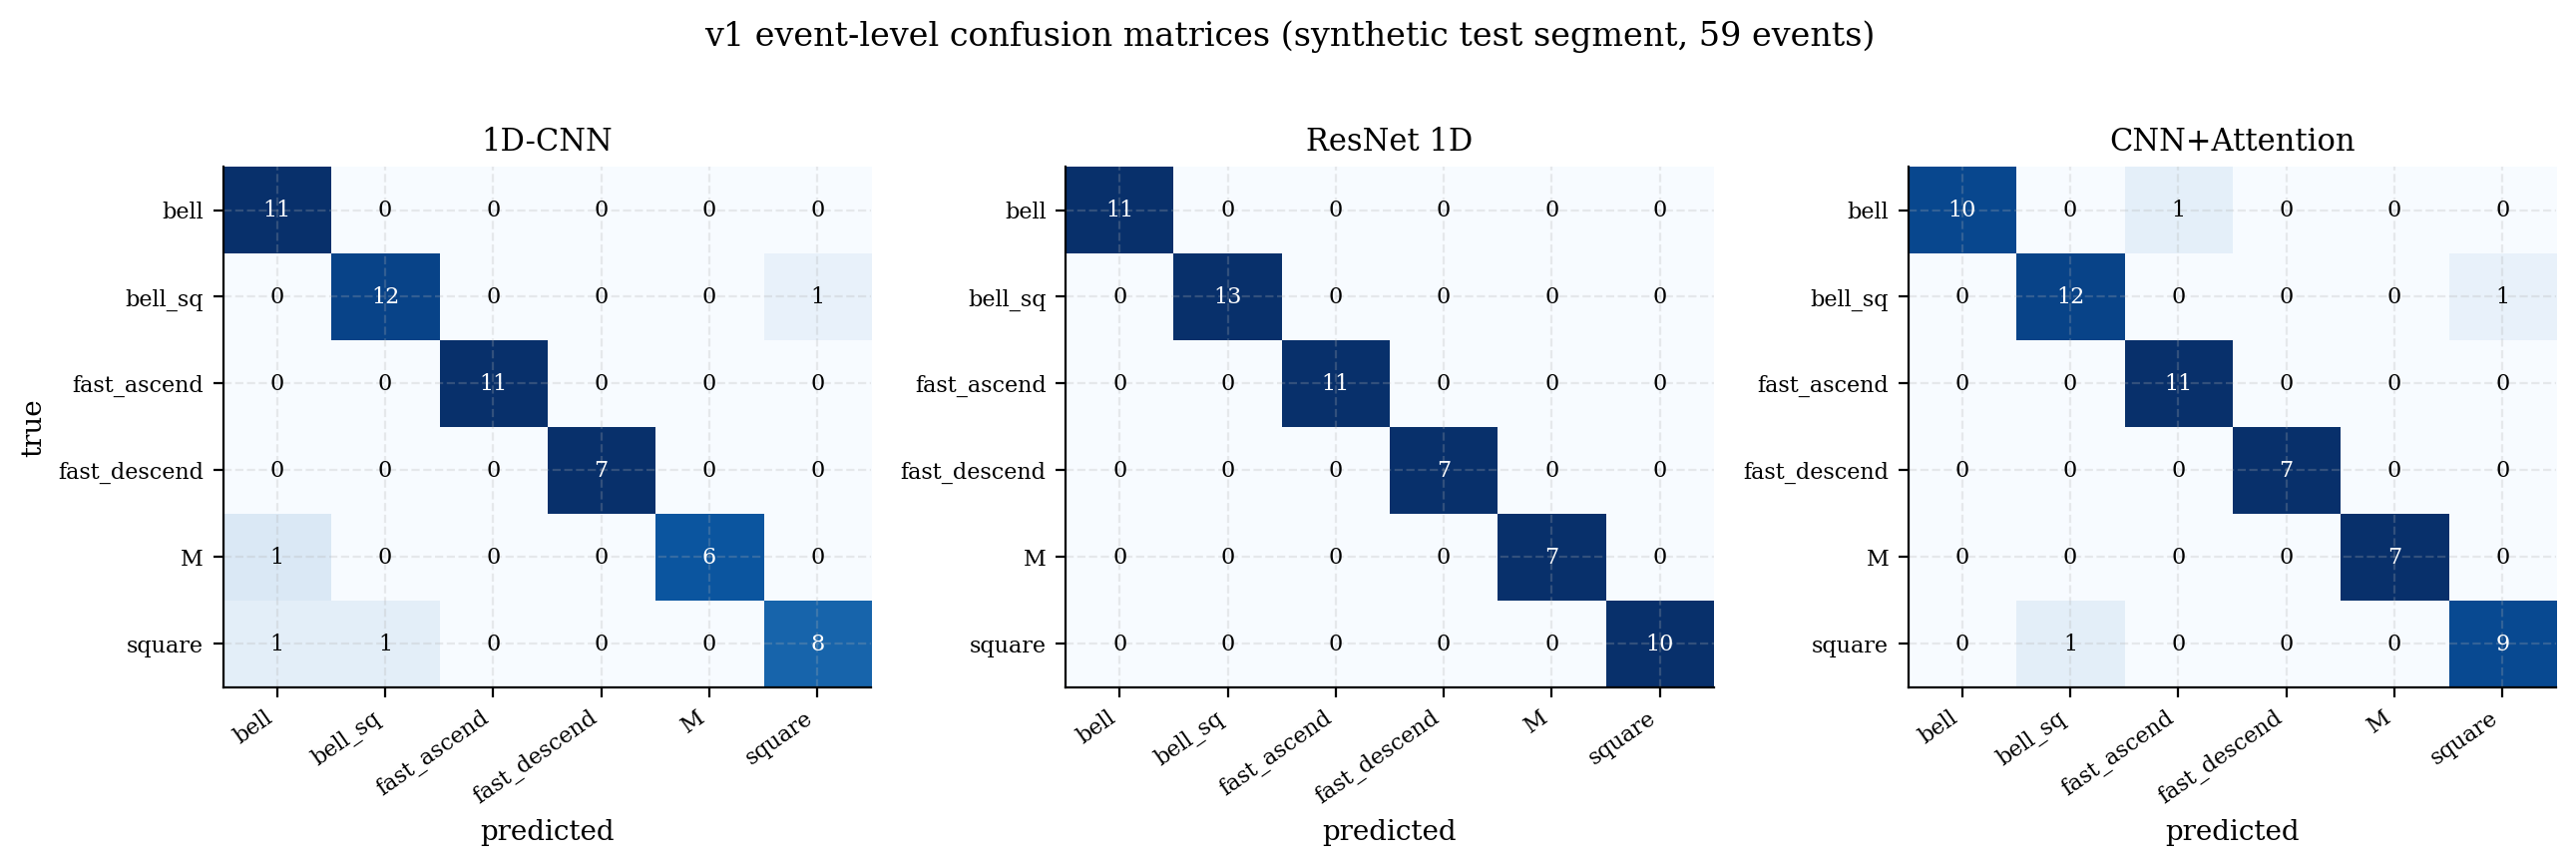
\includegraphics[width=\linewidth]{figures/v1_confusion_matrices}
    \caption{Event-level confusion matrices on the $59$-event synthetic segment.
    The ResNet is on the diagonal; the misses of the other two models fall on the
    visually similar morphologies.}
    \label{fig:confmat}
\end{figure}

\begin{table}[H]
    \centering \footnotesize
    \begin{tabular}{lccccc}
        \toprule
        Model & Hits & Misses & False alarms & Macro $P$ / $R$ & Macro $F_1$ \\
        \midrule
        1D-CNN        & 55 & 4 & 0 & 0.943 / 0.930 & 0.934 \\
        ResNet 1D     & 59 & 0 & 0 & 1.000 / 1.000 & \textbf{1.000} \\
        CNN+Attention & 56 & 3 & 0 & 0.957 / 0.955 & 0.955 \\
        \bottomrule
    \end{tabular}
    \caption{Event-level results on the synthetic segment ($59$ events).}
    \label{tab:event-f1}
\end{table}

\section{Robustness to distribution shift}
\label{sec:res-robust}

A deployed beacon will see conditions that differ from training. We stress each
model along two independent axes by regenerating small test sets (50 events each)
while varying one factor (\cref{fig:robust}): the background-noise level (the
noise std is multiplied by $m_{\mathrm{noise}}\in[1,3]$, and the anomaly
amplitude is scaled with it, so the test is one of \emph{noise texture and
normalisation}, not raw SNR) and the shape-deformation level
($\nu$ multiplied by $m_{\mathrm{deform}}\in[1,8]$). All models start at
$\sim 98\%$ $F_1$; \cref{tab:robust} reports where each falls below $50\%$.

\begin{figure}[H]
    \centering
    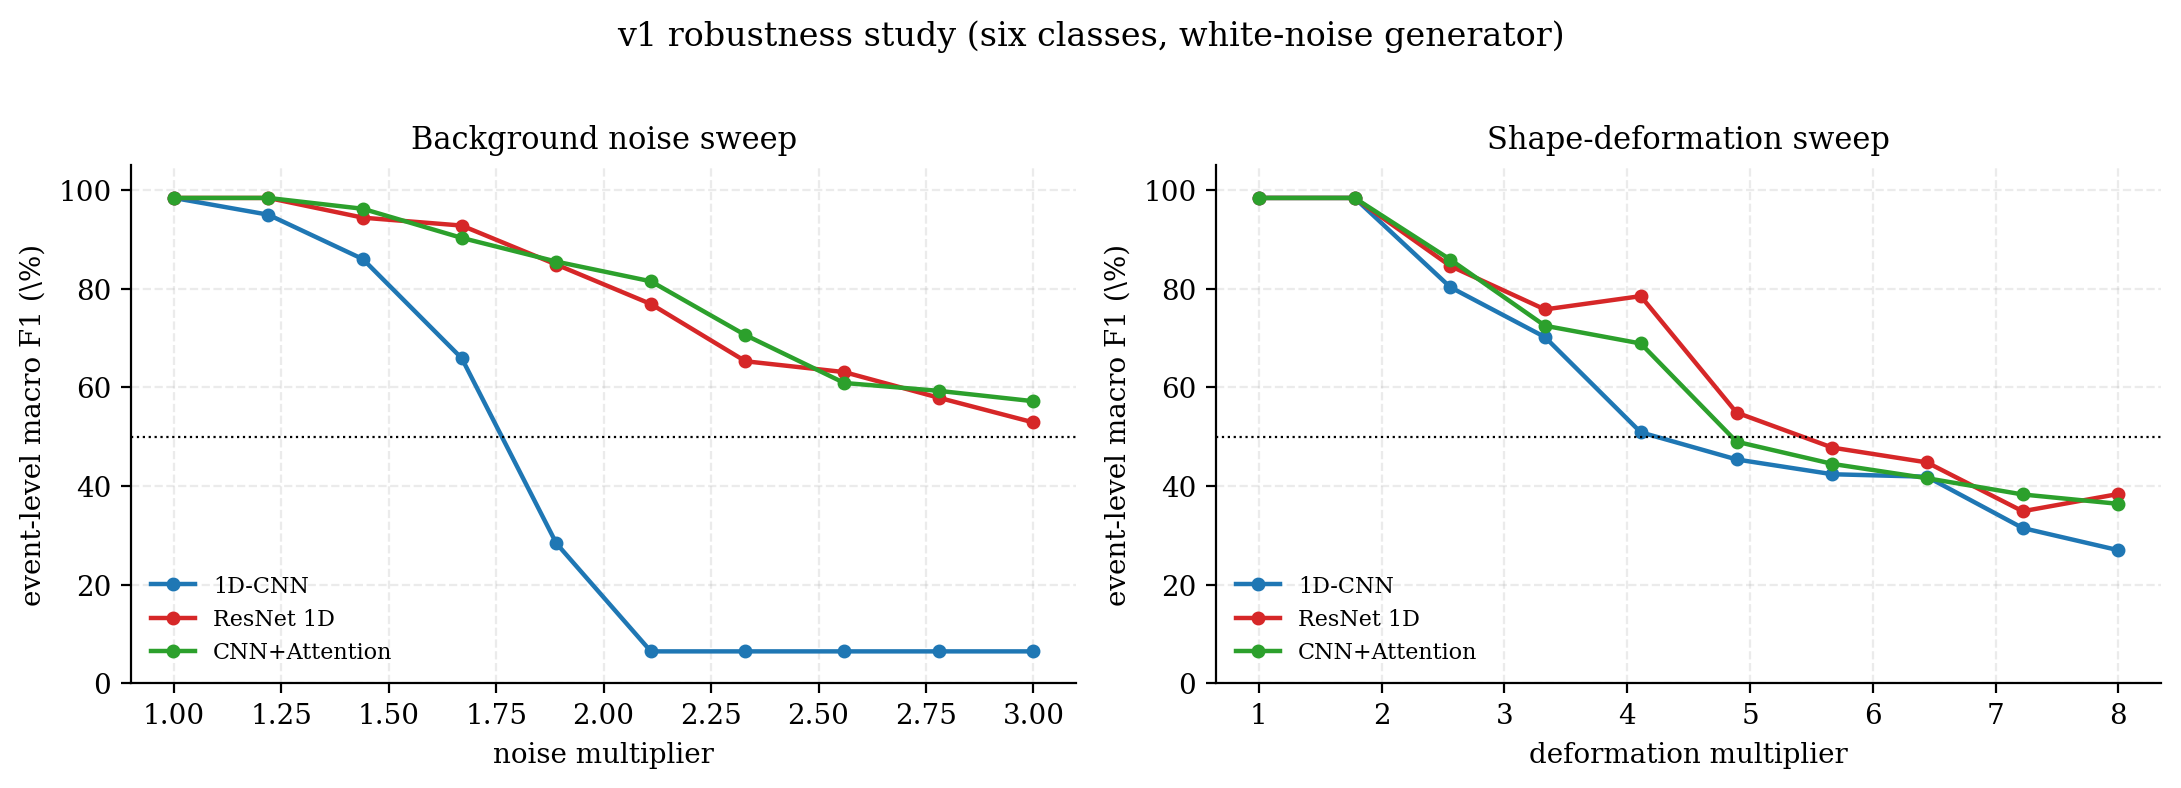
\includegraphics[width=\linewidth]{figures/v1_robustness}
    \caption{Robustness. Event-level macro $F_1$ vs background-noise multiplier
    (left) and vs shape-deformation multiplier (right).}
    \label{fig:robust}
\end{figure}

\begin{table}[H]
    \centering \footnotesize
    \begin{tabular}{lcc}
        \toprule
        Model & Noise: $F_1<50\%$ at & Deformation: $F_1<50\%$ at \\
        \midrule
        1D-CNN        & $m_{\mathrm{noise}}\approx 1.9$ (collapses to $\sim 6\%$) & $m_{\mathrm{deform}}\approx 4.9$ \\
        ResNet 1D     & never ($\geq 53\%$ up to $3\times$) & $m_{\mathrm{deform}}\approx 5.7$ \\
        CNN+Attention & never ($\geq 57\%$ up to $3\times$) & $m_{\mathrm{deform}}\approx 4.9$ \\
        \bottomrule
    \end{tabular}
    \caption{Robustness thresholds. The 1D-CNN collapses to a single class under
    moderate noise growth; the two group-norm models do not.}
    \label{tab:robust}
\end{table}

The contrast on the noise axis is stark: the baseline 1D-CNN drops below $50\%$
by $m_{\mathrm{noise}}\approx 1.9$ and then collapses to a single-class
$\sim 6\%$ plateau, whereas the ResNet and the CNN+Attention stay above $50\%$
across the whole sweep. The two robust models share group normalisation and skip
connections; the baseline's batch-norm running statistics, fitted at the training
noise level, become invalid as the input distribution shifts. On the
shape-deformation axis all three degrade gracefully, the ResNet most slowly.

\section{Computational cost}
\label{sec:res-cost}

\Cref{tab:cost} collects the cost--performance trade-off. The 1D-CNN is by far
the smallest and trains in a third of the time, but pays for it in accuracy and,
above all, noise robustness. The ResNet trains in about ten minutes on a laptop
GPU and gives the best accuracy, the best robustness and a perfect event-level
score, for a third of the parameters of the CNN+Attention. Inference is fast for
all three (thousands of windows per second); the throughput differences are small
and partly reflect first-run GPU warm-up for the baseline.

\begin{table}[H]
    \centering \footnotesize
    \begin{tabular}{lcccc}
        \toprule
        Model & Parameters & Train time & Inference (win/s) & Event $F_1$ \\
        \midrule
        1D-CNN        & $22{,}727$  & $\sim 4.3$ min & $\sim 10{,}700$ & 0.934 \\
        ResNet 1D     & $74{,}631$  & $\sim 10.0$ min & $\sim 14{,}200$ & \textbf{1.000} \\
        CNN+Attention & $109{,}655$ & $\sim 10.2$ min & $\sim 15{,}200$ & 0.955 \\
        \bottomrule
    \end{tabular}
    \caption{Cost vs performance (single RTX 5060 Laptop GPU).}
    \label{tab:cost}
\end{table}

\section{Discussion}
\label{sec:res-disc}

Three findings stand out. First, \textbf{residual learning with group
normalisation is the single biggest win}: at equal depth and an identical head,
the ResNet beats the plain 1D-CNN on every axis, and the gap explodes under
noise growth. Second, \textbf{self-attention buys no extra robustness here}: the
CNN+Attention sits between the other two, close to the ResNet but below it. The
$W=512$ window ($\le 800$-sample events) is short enough that a convolutional
receptive field already covers an event, leaving little long-range context for
attention to exploit --- we would expect attention to pay off on much longer
windows. Third, the \textbf{cheapest model is the most fragile}: the 1D-CNN's
single-class collapse under noise makes it unsuitable for a beacon that runs
across seasons. Overall the ResNet 1D is the best trade-off of accuracy,
robustness and cost on this benchmark.
